% !TeX program = pdflatex
% !TeX encoding = UTF-8
\documentclass[12pt,a4paper]{article}

\usepackage[utf8]{inputenc}
\usepackage[T1]{fontenc}
\usepackage{lmodern}
\usepackage[brazil]{babel}
\usepackage{listings}
\usepackage{xcolor}
\usepackage{graphicx}
\usepackage{float}
\usepackage{geometry}
\usepackage{indentfirst}
\usepackage{titlesec}
\usepackage{amsmath}
\usepackage{booktabs}
\usepackage{longtable}
\usepackage{tikz}
\usetikzlibrary{arrows.meta,positioning,fit}
\usepackage[hidelinks,pdftitle={Tarefa 12: Avaliação de Escalabilidade},pdfauthor={Matheus Bezeril Pinto}]{hyperref}

\geometry{a4paper,top=3cm,bottom=2cm,left=3cm,right=2cm}
\setlength{\parindent}{1.25cm}
\setlength{\parskip}{0.2cm}
\setlength{\emergencystretch}{2em}
\titleformat{\section}{\bfseries\large}{\thesection}{1em}{}
\titleformat{\subsection}{\bfseries\normalsize}{\thesubsection}{1em}{}
\graphicspath{{figuras/}}
\renewcommand{\lstlistingname}{Código}
\renewcommand{\lstlistlistingname}{Lista de códigos}
\definecolor{shellFont}{RGB}{233,233,233}
\definecolor{shellBG}{RGB}{44,51,122}
\definecolor{shellKeywords}{RGB}{250,227,0}
\definecolor{shellString}{RGB}{250,166,0}

\lstdefinestyle{Base}{
    basicstyle=\ttfamily\footnotesize,
    numbers=left,numberstyle=\tiny,numbersep=8pt,
    tabsize=4,breaklines=true,breakatwhitespace=false,
    showstringspaces=false,frame=single,
    columns=fullflexible,keepspaces=true,
    inputencoding=utf8,extendedchars=true,
    literate=
    {á}{{\'a}}1 {à}{{\`a}}1 {ã}{{\~a}}1 {â}{{\^a}}1
    {é}{{\'e}}1 {ê}{{\^e}}1 {í}{{\'i}}1
    {ó}{{\'o}}1 {ô}{{\^o}}1 {õ}{{\~o}}1
    {ú}{{\'u}}1 {ç}{{\c{c}}}1
    {Á}{{\'A}}1 {À}{{\`A}}1 {Ã}{{\~A}}1 {Â}{{\^A}}1
    {É}{{\'E}}1 {Ê}{{\^E}}1 {Í}{{\'I}}1
    {Ó}{{\'O}}1 {Ô}{{\^O}}1 {Õ}{{\~O}}1
    {Ú}{{\'U}}1 {Ç}{{\c{C}}}1
    {−}{{\ensuremath{-}}}1 {×}{{\ensuremath{\times}}}1
    {²}{{\ensuremath{^2}}}1
}
\lstdefinestyle{CStyle}{
    style=Base,language=C,
    keywordstyle=\color{blue}\bfseries,
    stringstyle=\color{red},
    commentstyle=\color{green!50!black},
    backgroundcolor=\color{gray!10}
}
\lstdefinestyle{Terminal}{
    style=Base,language=bash,
    basicstyle=\ttfamily\footnotesize\color{shellFont},
    keywordstyle=\color{shellKeywords}\bfseries,
    stringstyle=\color{shellString},
    commentstyle=\color{gray!30},
    numberstyle=\tiny\color{black},
    backgroundcolor=\color{shellBG}
}


\lstdefinestyle{Apendice}{
    style=CStyle,
    basicstyle=\fontsize{8.5}{10}\selectfont\ttfamily,
    numberstyle=\tiny,numbersep=7pt,
    backgroundcolor=\color{gray!4},
    xleftmargin=1em,framexleftmargin=.3em
}
\lstdefinestyle{Dados}{
    style=Apendice,language={},
    keywordstyle={},commentstyle={},stringstyle={},
    numbers=none,backgroundcolor=\color{white}
}

\title{\textbf{Tarefa 12: Avaliação de Escalabilidade}}
\author{Matheus Bezeril Pinto}
\date{Outubro de 2026}

\begin{document}
\maketitle

\section*{Resumo}
Este relatório avalia a escalabilidade do código de difusão viscosa da tarefa 11 em um nó de computação do NPAD. Foram comparadas três versões sucessivas em C com OpenMP: uma referência com região paralela a cada passo, uma versão com simplificação dos índices e uma versão com região paralela persistente. A campanha utilizou malhas de $200\times200$, $400\times400$ e $800\times800$, 2.000 passos, equipes de uma a dezesseis threads e cinco repetições por configuração, totalizando 225 medições. A referência alcançou speedup de $6{,}620$ e eficiência de $82{,}76\%$ com oito threads na maior malha. Com dezesseis threads, a eficiência caiu para $39{,}99\%$. Na avaliação fraca, o trabalho por thread foi mantido constante e a eficiência chegou a aproximadamente $38{,}9\%$ com dezesseis threads. As alterações produziram diferenças de tempo pequenas, sem uma melhoria expressiva e consistente. Os diagnósticos finais coincidiram entre versões e equipes. Os fontes, a configuração e os registros completos estão incluídos nos apêndices, permitindo avaliar o trabalho pelo próprio PDF.

\section{Objetivo e continuidade da tarefa 11}
A tarefa solicita avaliar a escalabilidade do código de Navier--Stokes em um nó do NPAD, identificar possíveis gargalos e relatar a evolução de versões otimizadas. O programa utilizado é o da tarefa 11: ele considera somente a difusão viscosa das componentes da velocidade. Portanto, os resultados caracterizam esse kernel e sua organização paralela; não representam uma solução completa de Navier--Stokes com pressão e advecção.

A implementação utiliza apenas os recursos de C e OpenMP já empregados nas tarefas anteriores: distribuição de laços, regiões paralelas, sincronização implícita e execução por lote. A organização dos experimentos segue os conceitos de escalabilidade forte e fraca apresentados até o slide que define a tarefa 12 \cite{slides}. As três versões são compiladas do mesmo conjunto de fontes, selecionando-se a macro \texttt{VERSAO}. A campanha analisada foi enviada ao repositório na revisão \texttt{99d6166} \cite{repositorio}.

\section{Modelo e trabalho computacional}
\subsection{Equações, discretização e campos}
No domínio periódico $[0,1)\times[0,1)$, são resolvidas as equações
\[
\frac{\partial u}{\partial t}=\nu\nabla^2u,
\qquad
\frac{\partial v}{\partial t}=\nu\nabla^2v,
\qquad \nu=0{,}01.
\]
Para uma componente $w$, o passo explícito é
\begin{equation}
\begin{split}
w^{n+1}_{i,j}=w^n_{i,j}
&+r_x(w^n_{i+1,j}-2w^n_{i,j}+w^n_{i-1,j})\\
&+r_y(w^n_{i,j+1}-2w^n_{i,j}+w^n_{i,j-1}),
\end{split}
\end{equation}
com $r_x=\nu\Delta t/\Delta x^2$ e $r_y=\nu\Delta t/\Delta y^2$. O código utiliza
\[
\Delta t=0{,}20\frac{\min(\Delta x^2,\Delta y^2)}{\nu},
\qquad \Delta x=1/N_x,\quad\Delta y=1/N_y.
\]
Assim, $r_x+r_y\leq0{,}40<0{,}50$, atendendo à condição de estabilidade da difusão explícita. As leituras são realizadas nos campos atuais; cada célula escreve exclusivamente nos campos do próximo passo. Ao final, trocam-se os ponteiros, sem copiar a malha inteira.

São mantidos quatro vetores de \texttt{double}: $u$, $v$, $u_{novo}$ e $v_{novo}$. A posição $(i,j)$ corresponde ao índice linear $iN_y+j$; o laço em $j$ percorre posições contíguas. Os vizinhos fora do domínio são obtidos por índices periódicos. Como cada iteração possui o mesmo tipo de cálculo, mantém-se \texttt{schedule(static)}, sem \texttt{collapse(2)}, em todas as versões. Isso evita misturar o efeito do schedule com o efeito das alterações avaliadas.

O modo 2 começa com $v=0$ e
\[
u(x,y,0)=1+0{,}5\exp\!\left[-\frac{(x-0{,}5)^2+(y-0{,}5)^2}{2(0{,}08)^2}\right].
\]
A perturbação se espalha pela difusão. Sua média positiva é conservada pelo domínio periódico; portanto, o estado uniforme limite não é exatamente $u=1$.

\subsection{Tamanho do problema}
Nesta campanha, $N_x=N_y=N$ e o número de passos é fixado em $K=2.000$. A quantidade de atualizações de células é
\begin{equation}
W=KN^2.
\label{eq:trabalho}
\end{equation}
Cada atualização evolui as duas componentes de velocidade. Essa contagem descreve trabalho algorítmico, não uma medição de operações de ponto flutuante ou de tráfego de memória.

\begin{table}[H]
\centering\small
\begin{tabular}{rrrrr}
\toprule
$N$ & $W$ (milhões) & Quatro vetores (MB) & $\Delta t$ & $t_{final}$\\
\midrule
200 & 80 & 1,28 & 0,00050000 & 1,0000\\
400 & 320 & 5,12 & 0,00012500 & 0,2500\\
800 & 1.280 & 20,48 & 0,00003125 & 0,0625\\
\bottomrule
\end{tabular}
\caption{Carga por execução e memória dos campos, considerando oito bytes por \texttt{double} e MB decimal. Não inclui estruturas auxiliares e bibliotecas.}
\label{tab:carga}
\end{table}

Fixar os passos permite comparar a evolução do custo por atualização. Entretanto, ao refinar a malha, o passo temporal estável diminui e o tempo físico final também diminui. Portanto, as três malhas não simulam a mesma duração física. Manter essa duração exigiria aumentar os passos aproximadamente com $N^2$, produzindo outro experimento, com trabalho proporcional a $N^4$ neste esquema explícito.

\section{Versões sucessivas da implementação}
\begin{figure}[H]
\centering
\begin{tikzpicture}[
  bloco/.style={draw=blue!60!black,fill=blue!5,rounded corners,
                text width=3.8cm,minimum height=2.1cm,align=center,font=\small},
  seta/.style={->,thick,blue!70!black}]
\node[bloco] (a) at (0,0) {\textbf{v0}\\[3pt]Kernel da tarefa 11\\Região paralela\\a cada passo};
\node[bloco] (b) at (4.9,0) {\textbf{v1}\\[3pt]Índices das linhas\\calculados fora\\do laço interno};
\node[bloco,fill=orange!12,draw=orange!70!black] (c) at (9.8,0)
{\textbf{v2}\\[3pt]Kernel de v1\\Uma região paralela\\para todos os passos};
\draw[seta] (a)--(b);
\draw[seta] (b)--(c);
\end{tikzpicture}
\caption{Evolução acumulada dos fontes. As três versões mantêm a mesma equação, a mesma ordem das operações por célula e o mesmo intervalo de medição.}
\label{fig:versoes}
\end{figure}


\subsection{v0: referência da tarefa 11}
A versão v0 conserva o cálculo dos índices e a ordem das operações por célula do kernel sem \texttt{collapse} da tarefa 11. Em cada passo, \texttt{compute\_next\_state} executa um \texttt{parallel for schedule(runtime)} sobre as linhas. Após o término dessa região, a função \texttt{swap\_fields} troca os ponteiros. O número de threads efetivamente participantes é registrado durante o laço.

Essa é a referência para avaliar o progresso entre versões. A compilação usa \texttt{-O3}, igualmente nas três versões, enquanto a campanha local da tarefa 11 havia usado outras condições e outro processador. Os tempos absolutos das duas tarefas não são uma comparação controlada de máquinas ou compiladores.

\subsection{v1: índices das linhas fora do laço interno}
Na v0, a obtenção dos índices das linhas vizinhas aparece no laço em $j$, embora dependa somente de $i$. A v1 explicita esse fato no fonte, calculando uma vez por linha:
\begin{lstlisting}[style=CStyle]
int row = i * sim->ny;
int previous_row = periodic(i - 1, sim->nx) * sim->ny;
int next_row = periodic(i + 1, sim->nx) * sim->ny;
\end{lstlisting}
No laço interno, os índices tornam-se somas entre essas bases e $j$. A organização das regiões paralelas permanece igual à da v0. A intenção é reduzir cálculos repetidos de endereçamento. Porém, um compilador com otimização já pode reconhecer parte dessas expressões invariantes; alterar o fonte não garante uma redução correspondente no código executado.

\subsection{v2: região paralela persistente}
A v2 mantém o kernel da v1, mas abre uma única região \texttt{parallel} para todos os passos. Dentro de \texttt{compute\_next\_state}, a diretiva passa a ser \texttt{omp for}, encontrada por todas as threads da equipe. A troca dos ponteiros fica em uma região \texttt{single}:
\begin{lstlisting}[style=CStyle]
#pragma omp parallel shared(sim)
{
    for (int step = 0; step < sim->steps; ++step)
    {
        compute_next_state(sim); /* contem omp for */
        #pragma omp single
        {
            swap_fields(sim);
        }
    }
}
\end{lstlisting}

O término do \texttt{omp for} possui uma barreira implícita: ninguém troca os campos enquanto outra thread ainda escreve no próximo estado. O término de \texttt{single} também possui uma barreira: ninguém começa o passo seguinte com os ponteiros ainda antigos. As duas sincronizações são necessárias nessa organização; não se utiliza \texttt{nowait}.

\begin{figure}[H]
\centering
\begin{tikzpicture}[
  etapa/.style={draw=blue!65!black,fill=blue!5,rounded corners,
                text width=2.7cm,minimum height=1.6cm,align=center,font=\small},
  seta/.style={->,thick}]
\node[etapa] (a) at (0,0) {\texttt{omp for}\\Todas as threads\\calculam o passo};
\node[etapa] (b) at (3.7,0) {Barreira\\implícita\\do \texttt{for}};
\node[etapa,fill=orange!15,draw=orange!70!black] (c) at (7.4,0)
{\texttt{single}\\Uma thread troca\\os ponteiros};
\node[etapa] (d) at (11.1,0) {Barreira\\implícita\\do \texttt{single}};
\draw[seta] (a)--(b);
\draw[seta] (b)--(c);
\draw[seta] (c)--(d);
\draw[seta] (d.north) -- ++(0,.8) -| node[pos=.25,above,font=\small]
{Próximo passo, com os campos completos} (a.north);
\node[draw=gray!60,dashed,rounded corners,fit=(a)(b)(c)(d),
      inner sep=9pt,label={[font=\small]below:Uma única região \texttt{parallel} em v2}] {};
\end{tikzpicture}
\caption{Sincronização preservada na versão persistente. O término do cálculo precede a troca dos campos, e a troca precede as leituras do passo seguinte.}
\label{fig:sincronizacao}
\end{figure}


A intenção é reduzir a entrada e a saída repetida de regiões paralelas. Isso não significa que v0 e v1 criem threads do sistema operacional novamente em cada passo: o runtime pode reutilizá-las. Além disso, a v2 continua pagando a sincronização a cada passo. Assim, a melhoria possível depende da relação entre esses custos e o trabalho da malha.

\section{Metodologia experimental no NPAD}
\subsection{Ambiente registrado}
A execução ocorreu em 18 de outubro de 2026, no nó \texttt{r1i1n15.npad.internal}, pelo job Slurm \texttt{2214966}, na partição \texttt{intel-128}. Foi solicitado um nó, uma tarefa e dezesseis CPUs para a tarefa. O ambiente registrado informa:
\begin{itemize}
\item Intel Xeon E5-2698 v3, frequência nominal de 2,30 GHz;
\item dois sockets, dezesseis núcleos por socket e duas threads de hardware por núcleo: 32 núcleos físicos e 64 CPUs lógicas no nó;
\item dois nós NUMA e cache L3 indicada pelo \texttt{lscpu} como \texttt{40960K};
\item GCC 8.5.0, identificação Red Hat \texttt{8.5.0-18}, Python 3.6.8 e Linux com kernel \texttt{4.18.0-477.10.1.el8\_8.x86\_64};
\item \texttt{OMP\_DYNAMIC=FALSE} e \texttt{OMP\_SCHEDULE=static}, sem módulos carregados.
\end{itemize}
Essas características descrevem o nó inteiro. A campanha não registrou a lista exata de CPUs atribuídas ao job nem o posicionamento de cada thread. Logo, dezesseis threads OpenMP não permitem concluir, isoladamente, que foram utilizados dezesseis núcleos físicos distintos. Não foi registrada a quantidade de RAM disponível; ela não é inferida do nome da partição.

\subsection{Compilação, submissão e repetições}
O script \texttt{compilar.sh} usa \texttt{-std=c11 -O3 -Wall -Wextra -fopenmp}, selecionando \texttt{-DVERSAO=0}, \texttt{1} ou \texttt{2}, e liga a biblioteca matemática. As três versões são compiladas dentro da pasta de resultados da própria campanha.

A execução foi submetida pelo script \texttt{jobs.sh}, que encaminha os argumentos para \texttt{sbatch submeter\_npad.sh}. O job executa \texttt{executar\_testes.sh} dentro da alocação, sem iniciar simulações no nó de login. Foram utilizados:
\begin{itemize}
\item três versões, três malhas e cinco equipes: $p\in\{1,2,4,8,16\}$;
\item modo 2, 2.000 passos e schedule estático em todas as combinações;
\item um aquecimento por configuração, descartado das estatísticas;
\item cinco execuções medidas por configuração, sem exclusão de amostras.
\end{itemize}
São $3\cdot3\cdot5=45$ configurações, 45 aquecimentos e 225 medições: 270 processos de simulação. As versões se alternam dentro da sequência de experimentos, mas os tamanhos e as equipes seguem uma ordem fixa. Essa organização reduz uma fonte de comparação desigual entre versões, porém não constitui aleatorização completa.

O conjunto recebido contém todas as 225 medições previstas, os 270 logs e o resumo final. Não foi fornecida uma saída final do \texttt{sacct}; a análise utiliza os registros completos da campanha, sem atribuir um tempo de fila ou uma duração total ao job.

\subsection{O que é cronometrado}
O programa mede com \texttt{omp\_get\_wtime()} apenas a chamada a \texttt{run\_simulation}. A alocação, a inicialização, os diagnósticos, a impressão e a gravação opcional do campo final ficam fora desse intervalo. Assim, os tempos incluem o cálculo, a distribuição do trabalho, as barreiras e a troca dos ponteiros, mas não a espera na fila Slurm ou a preparação da campanha.

O número efetivo de threads coincidiu com o solicitado em todas as medições. O script de análise calcula a média $\overline T$, o desvio padrão amostral $s$ e o coeficiente de variação
\[
s=\sqrt{\frac{\sum_{r=1}^{5}(T_r-\overline T)^2}{4}},
\qquad CV=100\frac{s}{\overline T}.
\]
As barras dos gráficos de tempo mostram um desvio padrão amostral, não um intervalo de confiança. O maior CV foi de aproximadamente $4{,}35\%$, na v0 com $N=800$ e duas threads. A maioria das configurações ficou abaixo de $2\%$.

\section{Métricas de escalabilidade}
\subsection{Escalabilidade forte}
Mantendo $N$ e $K$ fixos, aumenta-se somente o número de threads. Para cada versão $v$, definem-se
\begin{equation}
S_v(p,N)=\frac{\overline T_v(1,N)}{\overline T_v(p,N)},
\qquad
E_v(p,N)=\frac{S_v(p,N)}{p}.
\end{equation}
O comportamento ideal seria $S=p$ e $E=1$. A referência de uma thread é o mesmo executável OpenMP executado com uma thread, e não um programa sequencial independente. Cada versão usa sua própria referência para medir escalabilidade.

Para verificar se uma alteração melhorou o tempo absoluto, utiliza-se outra razão:
\[
G_v(p,N)=\frac{\overline T_{v0}(p,N)}{\overline T_v(p,N)}.
\]
Aqui a comparação preserva a malha e a equipe. Valores $G>1$ indicam vantagem sobre v0, e $G<1$ indicam tempo maior. Essa distinção evita confundir boa escalabilidade de uma versão com uma otimização efetiva em relação à referência.

\subsection{Escalabilidade fraca}
Mantendo $K$ fixo, mantém-se também o trabalho por thread:
\[
\frac{W}{p}=K\frac{N^2}{p}=\text{constante}.
\]
Para uma malha bidimensional, isso exige $N=N_0\sqrt p$. A diagonal disponível na campanha é
\[
(p,N)=(1,200),\ (4,400),\ (16,800).
\]
Essas combinações possuem 40.000 células e 80 milhões de atualizações por thread. Não há pontos fracos exatos para duas e oito threads nesta grade de tamanhos. A eficiência fraca é
\begin{equation}
E_{f,v}(p)=\frac{\overline T_v(1,200)}{\overline T_v(p,200\sqrt p)}.
\end{equation}
Idealmente, o tempo permanece constante e $E_f=1$. A grandeza que cresce linearmente com $p$ é o trabalho total $W$; o lado $N$ cresce com $\sqrt p$. Essa distinção é essencial ao aplicar o conceito de tamanho do problema a uma malha.

\begin{figure}[H]
\centering
\begin{tikzpicture}[font=\small]
\foreach \n [count=\c from 0] in {200,400,800}
  \node at (2.35*\c+1.1,.75) {$N=\n$};
\foreach \p [count=\r from 0] in {1,2,4,8,16}{
  \node[anchor=east] at (-.2,-.75*\r-.35) {$p=\p$};
  \foreach \n [count=\c from 0] in {200,400,800}{
    \fill[gray!4] (2.35*\c,-.75*\r) rectangle ++(2.2,-.68);
    \ifnum\p=1 \ifnum\c=0 \fill[orange!25] (2.35*\c,-.75*\r) rectangle ++(2.2,-.68);\fi\fi
    \ifnum\p=4 \ifnum\c=1 \fill[orange!25] (2.35*\c,-.75*\r) rectangle ++(2.2,-.68);\fi\fi
    \ifnum\p=16 \ifnum\c=2 \fill[orange!25] (2.35*\c,-.75*\r) rectangle ++(2.2,-.68);\fi\fi
    \draw[gray!50] (2.35*\c,-.75*\r) rectangle ++(2.2,-.68);
    \node at (2.35*\c+1.1,-.75*\r-.34) {$T(\p,\n)$};
  }
}
\draw[blue!75!black,very thick,rounded corners]
(4.62,.1) rectangle (6.98,-3.78);
\node[align=left,text width=11.8cm] at (3.2,-4.55)
{\textcolor{blue!75!black}{Contorno azul:} carga fixa, escalabilidade forte.\\
\colorbox{orange!25}{Diagonal laranja:} $N^2/p$ constante, escalabilidade fraca.};
\end{tikzpicture}
\caption{Cada versão produz uma matriz de tempos. A coluna fixa compara equipes na mesma malha; a diagonal compara $200^2/1=400^2/4=800^2/16$ células por thread.}
\label{fig:matriz}
\end{figure}


\section{Verificação dos resultados numéricos}
Todos os diagnósticos finais foram finitos. Para cada malha, as médias de $u$ e $v$, o máximo e o RMS da perturbação coincidiram nos valores registrados entre as três versões, todas as equipes e as cinco repetições. A componente $v$, inicialmente nula, continuou nula. As diferenças entre a média inicial e a final de $u$ foram inferiores a $2{,}3\times10^{-13}$ nas três malhas.

{\small\begin{longtable}{rrrrr}
\caption{Diagnósticos finais: para cada malha, idênticos em todas as versões e equipes.}\label{tab:diagnosticos}\\
\toprule $N$ & $t_{final}$ & Média de $u$ & Máximo & RMS\\
\midrule\endfirsthead
\toprule $N$ & $t_{final}$ & Média de $u$ & Máximo & RMS\\
\midrule\endhead
\bottomrule\endfoot
200 & 1,00000 & 1,020106192967 & 0,12117040 & 0,03491228\\
400 & 0,25000 & 1,020106192966 & 0,28065316 & 0,05312129\\
800 & 0,06250 & 1,020106192966 & 0,41827720 & 0,06484756\\
\end{longtable}
}

O máximo e o RMS são calculados a partir de $(u-1)^2+v^2$, pois o modo 2 usa a velocidade de referência $(1,0)$. A menor difusão observada na malha de 800 células por lado é coerente com seu menor tempo físico final, apresentado na Tabela~\ref{tab:carga}. Não é um indício de falha da paralelização.

A coincidência desses diagnósticos é uma verificação de consistência, mas não demonstra, sozinha, igualdade de todos os valores dos campos nem convergência para uma solução analítica. O script \texttt{validar.py}, incluído integralmente no apêndice, permite uma comparação célula a célula de campos salvos em uma execução de validação separada. Não se apresenta essa comparação como uma medição realizada nesta campanha quando o registro disponível contém apenas os diagnósticos.

\section{Resultados de escalabilidade forte}
\subsection{Maior malha: ganho até oito threads}
A Tabela~\ref{tab:forte} e a Figura~\ref{fig:forte} mostram os resultados para $800\times800$. Na v0, o tempo cai de $16{,}2869$ s com uma thread para $2{,}4601$ s com oito, com speedup $6{,}620$ e eficiência $82{,}76\%$. Com dezesseis threads, o tempo sobe para $2{,}5454$ s: o speedup passa a $6{,}399$ e a eficiência cai para $39{,}99\%$.

{\small\begin{longtable}{rrrrrrr}
\caption{Carga forte de $800\times800$, com 2.000 passos. Os índices indicam a versão.}\label{tab:forte}\\
\toprule $p$ & $T_0$ (s) & $S_0$ & $E_0$ (\%) & $T_1$ (s) & $T_2$ (s) & $E_2$ (\%)\\
\midrule\endfirsthead
\toprule $p$ & $T_0$ (s) & $S_0$ & $E_0$ (\%) & $T_1$ (s) & $T_2$ (s) & $E_2$ (\%)\\
\midrule\endhead
\bottomrule\endfoot
1 & 16,2869 & 1,000 & 100,00 & 16,2500 & 16,2246 & 100,00\\
2 & 8,4958 & 1,917 & 95,85 & 8,3817 & 8,4880 & 95,57\\
4 & 4,4202 & 3,685 & 92,12 & 4,4347 & 4,4347 & 91,46\\
8 & 2,4601 & 6,620 & 82,76 & 2,4704 & 2,4558 & 82,58\\
16 & 2,5454 & 6,399 & 39,99 & 2,5532 & 2,5539 & 39,71\\
\end{longtable}
}

\begin{figure}[H]
\centering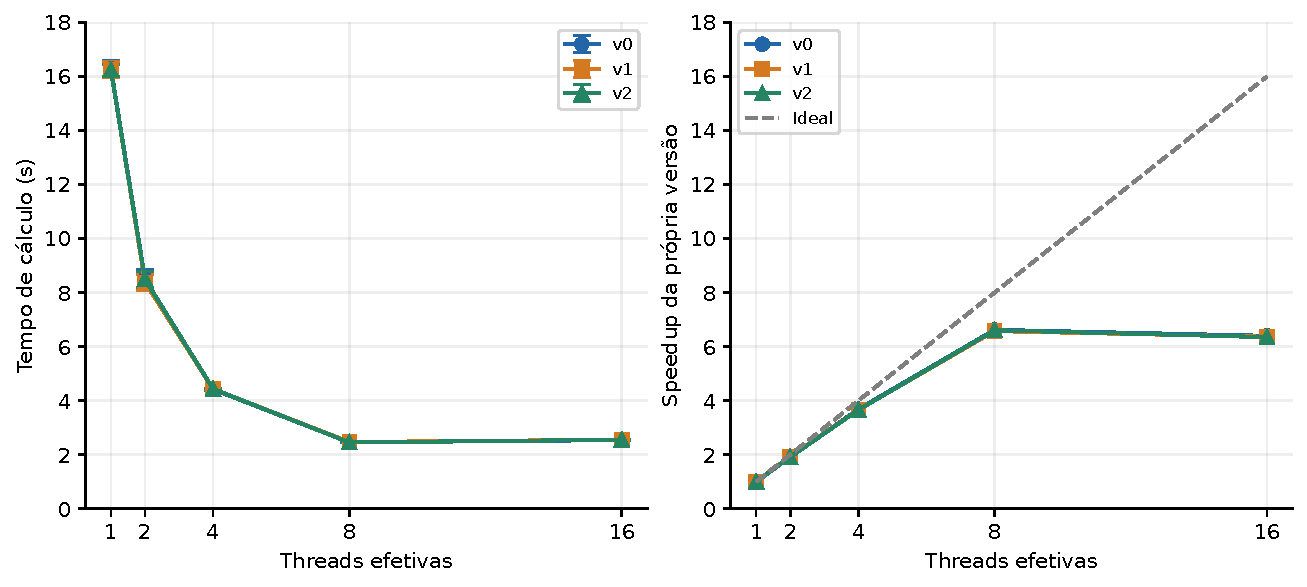
\includegraphics[width=\linewidth]{forte.pdf}
\caption{Escalabilidade forte em $800\times800$. As curvas das versões quase se sobrepõem; a linha tracejada indica speedup ideal. As barras de tempo representam um desvio padrão amostral.}
\label{fig:forte}
\end{figure}

As versões v1 e v2 apresentam a mesma tendência. A v2 atinge aproximadamente $2{,}4558$ s com oito threads e $2{,}5539$ s com dezesseis. Portanto, ampliar a equipe de oito para dezesseis threads não melhorou o tempo médio de nenhuma versão nessa malha.

\subsection{Influência do tamanho da malha}
\begin{figure}[H]
\centering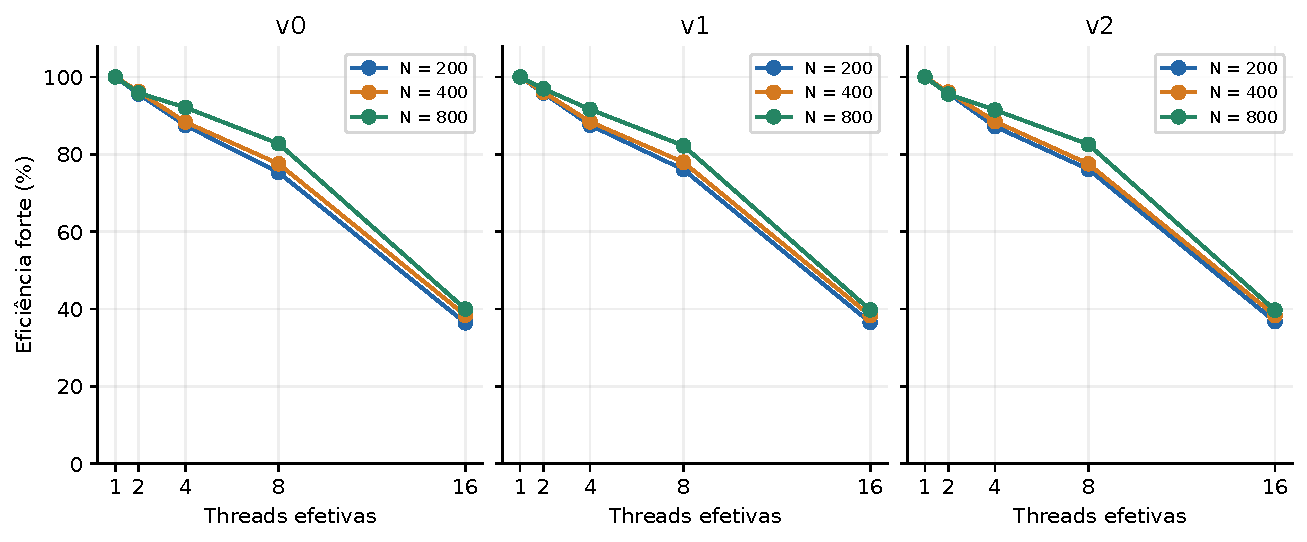
\includegraphics[width=\linewidth]{eficiencia.pdf}
\caption{Eficiência forte para cada versão e tamanho de malha. O trabalho adicional nas malhas maiores ajuda a amortizar custos paralelos, mas não elimina a perda de eficiência em dezesseis threads.}
\label{fig:eficiencia}
\end{figure}

Na v0 com oito threads, a eficiência sobe de aproximadamente $75{,}29\%$ em $N=200$ para $77{,}54\%$ em $N=400$ e $82{,}76\%$ em $N=800$. A tendência é compatível com maior quantidade de trabalho útil por distribuição do laço e por sincronização. Mesmo assim, todas as nove combinações de versão e malha tiveram o menor tempo médio com oito threads. Em dezesseis threads, as eficiências ficam aproximadamente entre $36\%$ e $40\%$.

Esses resultados indicam um limite prático na configuração medida, e não uma proibição geral de usar dezesseis threads. Outra alocação de CPUs, outro nó ou uma carga diferente podem produzir outro comportamento.

\section{Resultados de escalabilidade fraca}
{\small\begin{longtable}{lrrrrr}
\caption{Escalabilidade fraca: 80 milhões de atualizações de células por thread.}\label{tab:fraca}\\
\toprule Versão & $p$ & $N$ & Média (s) & $s$ (s) & $E_f$ (\%)\\
\midrule\endfirsthead
\toprule Versão & $p$ & $N$ & Média (s) & $s$ (s) & $E_f$ (\%)\\
\midrule\endhead
\bottomrule\endfoot
v0 & 1 & 200 & 0,989695 & 0,001838 & 100,00\\
v0 & 4 & 400 & 1,116827 & 0,002938 & 88,62\\
v0 & 16 & 800 & 2,545390 & 0,000510 & 38,88\\
v1 & 1 & 200 & 0,989874 & 0,001580 & 100,00\\
v1 & 4 & 400 & 1,114764 & 0,001485 & 88,80\\
v1 & 16 & 800 & 2,553170 & 0,001979 & 38,77\\
v2 & 1 & 200 & 0,988254 & 0,001145 & 100,00\\
v2 & 4 & 400 & 1,113601 & 0,005839 & 88,74\\
v2 & 16 & 800 & 2,553923 & 0,000540 & 38,70\\
\end{longtable}
}

\begin{figure}[H]
\centering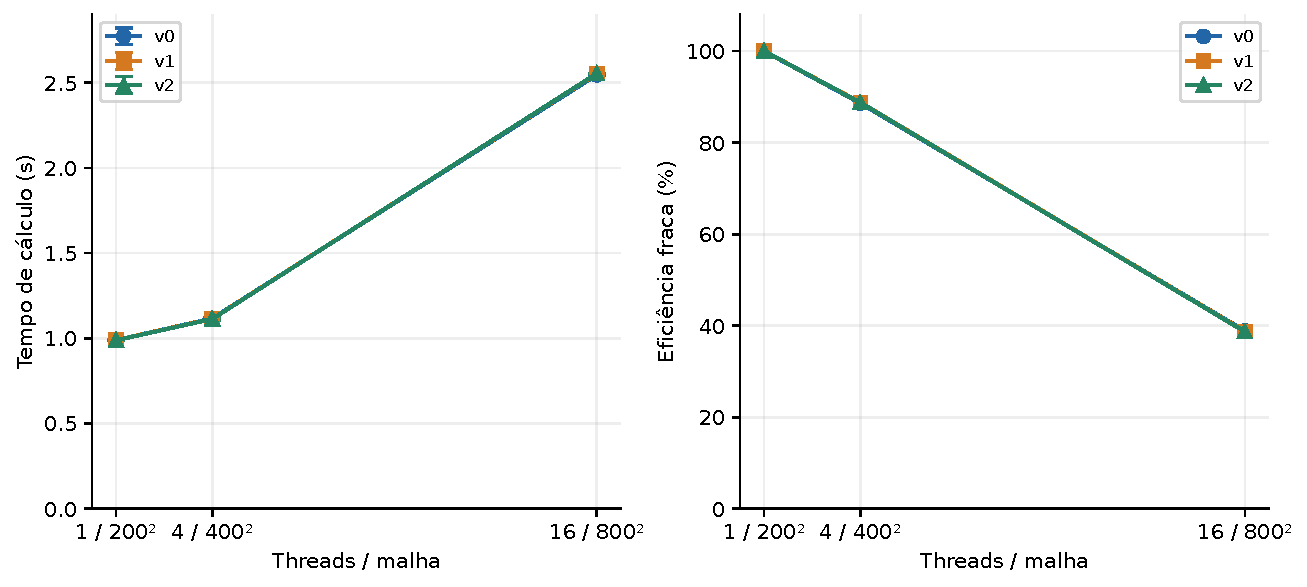
\includegraphics[width=\linewidth]{fraca.pdf}
\caption{Escalabilidade fraca com trabalho por thread constante. O tempo ideal seria horizontal, próximo de um segundo, e a eficiência ideal permaneceria em $100\%$.}
\label{fig:fraca}
\end{figure}

Na v0, aumentar simultaneamente a equipe e a malha leva o tempo de $0{,}9897$ s em $(1,200)$ para $1{,}1168$ s em $(4,400)$ e $2{,}5454$ s em $(16,800)$. As eficiências fracas correspondentes são $88{,}62\%$ e $38{,}88\%$. A v1 e a v2 ficam muito próximas: aproximadamente $88{,}8\%$ com quatro threads e $38{,}7\%$ com dezesseis.

Assim, a configuração apresenta escalabilidade fraca razoável até o ponto de quatro threads, com perda de cerca de $11\%$ de eficiência, mas uma degradação acentuada no ponto de dezesseis. O fato de a carga por thread permanecer constante não mantém constantes a pressão sobre recursos compartilhados nem todos os custos de coordenação.

Este resultado complementa a avaliação forte: aumentar o problema na proporção do número de threads também não recuperou boa eficiência em dezesseis threads. Como a diagonal contém apenas três pontos, não se caracteriza uma curva contínua nem se extrapola o comportamento para equipes maiores.

\section{Progresso das versões e possíveis gargalos}
\subsection{As alterações não produziram ganho expressivo}
\begin{figure}[H]
\centering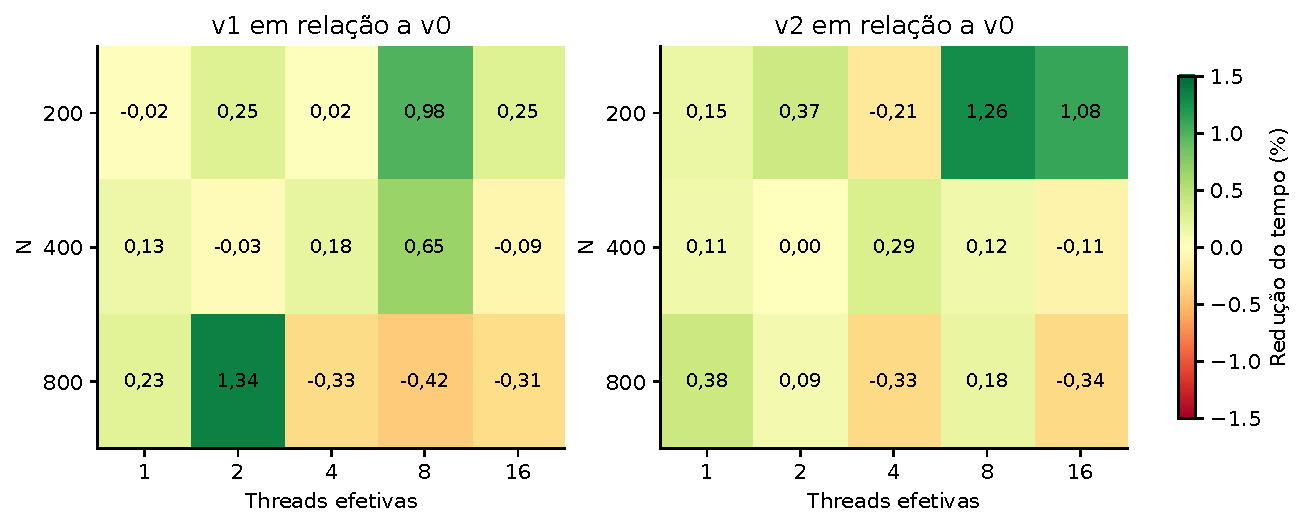
\includegraphics[width=\linewidth]{ganho.pdf}
\caption{Redução percentual do tempo médio em relação à v0, com a mesma malha e equipe. Valores positivos indicam tempo menor; valores negativos indicam tempo maior. A escala evidencia diferenças pequenas.}
\label{fig:ganho}
\end{figure}

Na v1, a razão $G$ varia aproximadamente de $0{,}9958$ a $1{,}0136$; na v2, de $0{,}9967$ a $1{,}0128$. Em termos de redução do tempo, o maior ganho observado fica em torno de $1{,}3\%$, e há configurações ligeiramente mais lentas. Algumas diferenças têm a mesma ordem da dispersão das cinco repetições. Sem uma análise estatística adicional e uma campanha direcionada, não se atribui superioridade geral a uma das versões.

O progresso foi, portanto, implementar e avaliar duas mudanças controladas, preservando os resultados numéricos, e verificar que elas não alteraram substancialmente o desempenho neste experimento. A v1 torna explícito um cálculo invariante que o GCC pode já otimizar. Na v2, o custo evitado de regiões paralelas repetidas pode ser pequeno diante do trabalho da malha e das sincronizações que continuam necessárias. São explicações plausíveis, não conclusões obtidas de inspeção do código de máquina ou de um perfil de execução.

\subsection{Gargalo observado e limites da identificação}
O principal comportamento observado é a saturação a partir de oito threads: o dobro de threads não produz redução do tempo. O kernel realiza atualizações regulares com acessos a campos e vizinhos; os candidatos a explicar essa saturação incluem o compartilhamento de recursos de memória/cache, a organização das CPUs efetivamente alocadas e o custo de coordenação da equipe.

Há, entretanto, limites concretos na evidência disponível:
\begin{itemize}
\item não foram medidos largura de banda, faltas de cache ou tempo gasto nas barreiras;
\item o registro do hardware informa duas threads por núcleo, mas não associa as threads do job a núcleos físicos específicos;
\item os quatro vetores da maior malha ocupam cerca de 20,48 MB, porém isso não demonstra que todos os acessos sejam atendidos por uma cache específica;
\item não foi feito um levantamento da concorrência de outros jobs por recursos do nó.
\end{itemize}
Portanto, o relatório identifica o ponto de perda de escalabilidade e apresenta hipóteses compatíveis com o algoritmo, sem afirmar que foi comprovado um gargalo exclusivo de memória, de NUMA ou de sincronização. O schedule estático é coerente com o trabalho uniforme por célula; não há evidência, nos tempos coletados, de que um desbalanceamento algorítmico seja o fator principal.

Uma continuação experimental útil seria repetir a configuração de oito e dezesseis threads registrando a alocação efetiva de CPUs e ampliar as repetições para separar diferenças pequenas entre versões. Não é necessário introduzir novos mecanismos de paralelização para reconhecer os limites desta campanha.

\section{Conclusão}
O código foi executado em um nó de computação do NPAD e avaliado sob carga fixa e sob trabalho por thread constante. A campanha completa contém 225 medições e apresenta diagnósticos finais consistentes entre versões e equipes. Na maior malha, a referência alcançou speedup $6{,}620$ e eficiência $82{,}76\%$ com oito threads. Esse foi o melhor tamanho de equipe entre os avaliados para todas as versões e malhas.

Com dezesseis threads, a eficiência forte caiu para aproximadamente $36\%$ a $40\%$, e a eficiência fraca ficou próxima de $39\%$. As duas alterações implementadas não removeram esse limite nem proporcionaram uma melhoria expressiva e consistente de tempo. O resultado reforça que uma alteração aparentemente favorável no fonte precisa ser confirmada por medições, e que aumentar a equipe não garante reduzir o tempo de execução.

As conclusões ficam restritas ao modelo viscoso, às cargas medidas e à alocação utilizada. Os apêndices documentam integralmente os programas, os scripts, as estatísticas, o ambiente e os logs, permitindo conferir a análise sem acesso ao GitHub ou a arquivos anexos separados.

\clearpage
\appendix
\section{Reprodução e organização do material}
O projeto LaTeX possui preâmbulo completo, ilustrações TikZ, figuras e tabelas já geradas. Sua compilação com pdfLaTeX não executa Python nem os experimentos. Os comandos \texttt{\textbackslash lstinputlisting} incluem os arquivos completos de \texttt{codigos/}, sem limites de linhas. Esses arquivos são cópias dos fontes efetivamente analisados, separadas da versão principal para manter o relatório reprodutível.

No NPAD, a partir da pasta principal \texttt{Tarefa\_12}, a submissão padrão é:
\begin{lstlisting}[style=Terminal]
bash jobs.sh
\end{lstlisting}
Os parâmetros de fila e alocação estão em \texttt{submeter\_npad.sh}. A execução só deve ocorrer após a alocação do Slurm. Para esta campanha, o resultado foi armazenado em \texttt{resultados/execucao\_20261018T180336Z\_38920/}. Acompanhar a execução com \texttt{squeue} e confirmar o término com \texttt{sacct} evita copiar resultados enquanto ainda estão sendo escritos.

O PDF contém o material utilizado para a análise: códigos completos, 45 resumos estatísticos, configuração, ambiente, hashes, log de compilação e as 270 saídas de execução. Os 225 tempos brutos e os diagnósticos aparecem nessas saídas, além das cópias CSV que acompanham o projeto. Os aquecimentos estão identificados por \texttt{aquecimento} e não entram nas médias. As figuras apresentam os dados sem omitir configurações mais lentas.

\section{Programas e scripts completos}
\subsection{Estruturas e interface: fluid.h}
\lstinputlisting[style=Apendice]{codigos/fluid.h}
\clearpage\subsection{Programa principal: fluid\_sim.c}
\lstinputlisting[style=Apendice]{codigos/fluid_sim.c}
\clearpage\subsection{Simulação e versões: fluid.c}
\lstinputlisting[style=Apendice]{codigos/fluid.c}
\clearpage\subsection{Compilação: compilar.sh}
\lstinputlisting[style=Apendice,language=bash]{codigos/compilar.sh}
\subsection{Entrada da submissão: jobs.sh}
\lstinputlisting[style=Apendice,language=bash]{codigos/jobs.sh}
\subsection{Job Slurm: submeter\_npad.sh}
\lstinputlisting[style=Apendice,language=bash]{codigos/submeter_npad.sh}
\clearpage\subsection{Campanha: executar\_testes.sh}
\lstinputlisting[style=Apendice,language=bash]{codigos/executar_testes.sh}
\clearpage\subsection{Análise: analisar\_resultados.py}
\lstinputlisting[style=Apendice,language=Python]{codigos/analisar_resultados.py}
\clearpage\subsection{Validação célula a célula: validar.py}
Este utilitário é fornecido para a validação separada; sua inclusão não acrescenta medições à campanha de desempenho.
\lstinputlisting[style=Apendice,language=Python]{codigos/validar.py}

\clearpage\section{Resultados completos e registros do ambiente}
{\scriptsize\setlength{\tabcolsep}{3pt}\begin{longtable}{lrrrrrrrr}
\caption{Todas as 45 configurações, com cinco repetições cada. $S$ e $E$ usam a própria versão; $G$ usa v0 com a mesma carga e equipe.}\label{tab:completo}\\
\toprule Versão & $N$ & $p$ & Média (s) & $s$ (s) & CV (\%) & $S$ & $E$ (\%) & $G$\\
\midrule\endfirsthead
\toprule Versão & $N$ & $p$ & Média (s) & $s$ (s) & CV (\%) & $S$ & $E$ (\%) & $G$\\
\midrule\endhead
\bottomrule\endfoot
v0 & 200 & 1 & 0,989695 & 0,001838 & 0,19 & 1,000 & 100,00 & 1,0000\\
v0 & 200 & 2 & 0,517672 & 0,001563 & 0,30 & 1,912 & 95,59 & 1,0000\\
v0 & 200 & 4 & 0,282755 & 0,000407 & 0,14 & 3,500 & 87,50 & 1,0000\\
v0 & 200 & 8 & 0,164318 & 0,002955 & 1,80 & 6,023 & 75,29 & 1,0000\\
v0 & 200 & 16 & 0,169786 & 0,000267 & 0,16 & 5,829 & 36,43 & 1,0000\\
v0 & 400 & 1 & 3,946659 & 0,003730 & 0,09 & 1,000 & 100,00 & 1,0000\\
v0 & 400 & 2 & 2,051163 & 0,012509 & 0,61 & 1,924 & 96,21 & 1,0000\\
v0 & 400 & 4 & 1,116827 & 0,002938 & 0,26 & 3,534 & 88,35 & 1,0000\\
v0 & 400 & 8 & 0,636243 & 0,007254 & 1,14 & 6,203 & 77,54 & 1,0000\\
v0 & 400 & 16 & 0,642273 & 0,000187 & 0,03 & 6,145 & 38,41 & 1,0000\\
v0 & 800 & 1 & 16,286901 & 0,308834 & 1,90 & 1,000 & 100,00 & 1,0000\\
v0 & 800 & 2 & 8,495826 & 0,369292 & 4,35 & 1,917 & 95,85 & 1,0000\\
v0 & 800 & 4 & 4,420166 & 0,048040 & 1,09 & 3,685 & 92,12 & 1,0000\\
v0 & 800 & 8 & 2,460088 & 0,001825 & 0,07 & 6,620 & 82,76 & 1,0000\\
v0 & 800 & 16 & 2,545390 & 0,000510 & 0,02 & 6,399 & 39,99 & 1,0000\\
v1 & 200 & 1 & 0,989874 & 0,001580 & 0,16 & 1,000 & 100,00 & 0,9998\\
v1 & 200 & 2 & 0,516397 & 0,001368 & 0,26 & 1,917 & 95,84 & 1,0025\\
v1 & 200 & 4 & 0,282709 & 0,000839 & 0,30 & 3,501 & 87,53 & 1,0002\\
v1 & 200 & 8 & 0,162715 & 0,002276 & 1,40 & 6,083 & 76,04 & 1,0099\\
v1 & 200 & 16 & 0,169364 & 0,000337 & 0,20 & 5,845 & 36,53 & 1,0025\\
v1 & 400 & 1 & 3,941437 & 0,005004 & 0,13 & 1,000 & 100,00 & 1,0013\\
v1 & 400 & 2 & 2,051850 & 0,001017 & 0,05 & 1,921 & 96,05 & 0,9997\\
v1 & 400 & 4 & 1,114764 & 0,001485 & 0,13 & 3,536 & 88,39 & 1,0019\\
v1 & 400 & 8 & 0,632081 & 0,009544 & 1,51 & 6,236 & 77,95 & 1,0066\\
v1 & 400 & 16 & 0,642851 & 0,000308 & 0,05 & 6,131 & 38,32 & 0,9991\\
v1 & 800 & 1 & 16,249956 & 0,298899 & 1,84 & 1,000 & 100,00 & 1,0023\\
v1 & 800 & 2 & 8,381656 & 0,295930 & 3,53 & 1,939 & 96,94 & 1,0136\\
v1 & 800 & 4 & 4,434661 & 0,004417 & 0,10 & 3,664 & 91,61 & 0,9967\\
v1 & 800 & 8 & 2,470359 & 0,023442 & 0,95 & 6,578 & 82,22 & 0,9958\\
v1 & 800 & 16 & 2,553170 & 0,001979 & 0,08 & 6,365 & 39,78 & 0,9970\\
v2 & 200 & 1 & 0,988254 & 0,001145 & 0,12 & 1,000 & 100,00 & 1,0015\\
v2 & 200 & 2 & 0,515768 & 0,000817 & 0,16 & 1,916 & 95,80 & 1,0037\\
v2 & 200 & 4 & 0,283351 & 0,001458 & 0,51 & 3,488 & 87,19 & 0,9979\\
v2 & 200 & 8 & 0,162249 & 0,002857 & 1,76 & 6,091 & 76,14 & 1,0128\\
v2 & 200 & 16 & 0,167948 & 0,000230 & 0,14 & 5,884 & 36,78 & 1,0109\\
v2 & 400 & 1 & 3,942177 & 0,002404 & 0,06 & 1,000 & 100,00 & 1,0011\\
v2 & 400 & 2 & 2,051088 & 0,001947 & 0,09 & 1,922 & 96,10 & 1,0000\\
v2 & 400 & 4 & 1,113601 & 0,005839 & 0,52 & 3,540 & 88,50 & 1,0029\\
v2 & 400 & 8 & 0,635510 & 0,006449 & 1,01 & 6,203 & 77,54 & 1,0012\\
v2 & 400 & 16 & 0,642967 & 0,000195 & 0,03 & 6,131 & 38,32 & 0,9989\\
v2 & 800 & 1 & 16,224628 & 0,209850 & 1,29 & 1,000 & 100,00 & 1,0038\\
v2 & 800 & 2 & 8,488001 & 0,289683 & 3,41 & 1,911 & 95,57 & 1,0009\\
v2 & 800 & 4 & 4,434724 & 0,002633 & 0,06 & 3,659 & 91,46 & 0,9967\\
v2 & 800 & 8 & 2,455765 & 0,004148 & 0,17 & 6,607 & 82,58 & 1,0018\\
v2 & 800 & 16 & 2,553923 & 0,000540 & 0,02 & 6,353 & 39,71 & 0,9967\\
\end{longtable}
}
\subsection{Configuração da campanha}
\lstinputlisting[style=Dados]{dados/configuracao.json}
\subsection{Critérios registrados pelo analisador}
\lstinputlisting[style=Dados]{dados/observacoes.txt}
\clearpage\subsection{Ambiente registrado no nó de computação}
\lstinputlisting[style=Dados]{dados/ambiente.txt}
\subsection{Identificação dos fontes por SHA-256}
Os hashes abaixo identificam os arquivos utilizados pela campanha; o gerador do relatório é posterior e não faz parte desses hashes.
\lstinputlisting[style=Dados]{dados/fontes.sha256}
\subsection{Registro de compilação}
\lstinputlisting[style=Dados]{dados/compilacao.log}

\clearpage\section{Código completo de geração das figuras e tabelas}
O script lê somente os dados incluídos, confere as médias e os desvios contra os tempos brutos e gera os artefatos gráficos. Requer NumPy e Matplotlib apenas para regenerá-los.
\lstinputlisting[style=Apendice,language=Python]{gerar_figuras.py}

\clearpage\section{Saídas integrais das execuções}
As saídas estão organizadas por versão, malha e equipe. Para cada configuração, aparece primeiro o aquecimento e depois as cinco repetições. Cada cabeçalho preserva o nome original do arquivo. Nenhuma linha de saída das simulações foi suprimida. A quebra visual das linhas longas não altera seu conteúdo.
\lstinputlisting[style=Dados]{dados/logs_completos.txt}

\clearpage
\begin{thebibliography}{9}
\bibitem{slides} Material da disciplina de Programação Paralela. \textit{SlidesAulas.pdf}, conteúdo até a definição da Tarefa 12, página 55 do PDF (slide numerado 57). Material disponibilizado pelo professor.
\bibitem{repositorio} PINTO, Matheus Bezeril. \textit{ProgParalela2026.2: Tarefas 11 e 12}. Fontes e campanha NPAD analisados na revisão \texttt{99d6166}. Disponível em: \url{https://github.com/39Matheus/ProgParalela2026.2}. Os arquivos necessários à leitura dos resultados estão reproduzidos neste relatório.
\bibitem{openmp} OpenMP Architecture Review Board. \textit{OpenMP Application Programming Interface}. Documentação de regiões paralelas, worksharing, single e barreiras implícitas. Disponível em: \url{https://www.openmp.org/specifications/}.
\end{thebibliography}
\end{document}
